\chapter{Router security}

Three areas of router security must be maintained:

\begin{itemize}
\item \textbf{Physical security:} Place the router and physical devices that connect to it in a secure locked and dedicated room 

\item \textbf{Operating system security:} Configure the router with the maximum amount of memory possible, Use the latest, stable version of the operating system, Keep a secure copy of router operating system images and router configuration files

\item \textbf{Router Hardening:} Secure administrative access, Disable unnecessary ports, interfaces and services
\end{itemize}


\section{Administrative access}
%
%\paragraph{Type of management access:} 
%
%When logging and managing information, the information flow between management hosts and the managed devices can take two paths: In-band (SSH, SNMP, etc.) and Out-of-band (console port). Out-of-band management is appropriate for large enterprise networks, because it remains unaffected by the downed link. In-band management is recommended in smaller networks as a means of achieving a more cost-effective security deployment.
%
%\paragraph{Strong password:} 
%
%To create a strong password, use a blank space in the password (only password-leading spaces are ignored) or create a phrase made of many words. This is called a \emph{passphrase}. A passphrase is often easier to remember than a complex password and more difficult to guess.
%
%\paragraph{Secret Password Algorithms:} 

\subsection{Virtual logins}

All passwords in Cisco IOS uses an MD5 hash by default. However, MD5 hashes are no longer considered secure. Therefore, it is now recommended that you configure all passwords using either type 8 \code{sha256} or type 9 \code{scrypt} passwords.

\begin{sexylisting}{Secret password type 9}
enable algorithm-type scrypt secret cisco12345
username Huy algorithm-type scrypt secret cisco12345
\end{sexylisting}

The following Cisco IOS login enhancements commands increase the security of virtual login connections.

\begin{sexylisting}{Login security commands}
login block-for 15 attempts 5 within 60
login quite-mode access-class PERMIT-ADMIN
login delay 10
login on-access log
login on-failure log
end
show login
show login failures
\end{sexylisting}

The \code{login block-for} command disables logins for 60 seconds if more than 5 login failures occur within 15 seconds. Doing this can defend against DoS attacks. The \code{login delay} command specifies a number of seconds the user must wait between unsuccessful login attempts. The \code{login on-success} and \code{login on-failure} commands generate syslog messages for successful and unsuccessful login attempts. The \code{security auth failure rate} command can be configured to generate a log message when the login failure rate is exceeded.\\

Note that these login enhancements do \emph{not} apply to console connections and only available if local database is used for authentication. If the lines are configured for password authentication only, then the enhanced login features are not enabled.

%\subsection{Configuring SSH}
%
%There are four requirements the router must meet before configuring SSH:
%
%\begin{itemize}
%\item Runs a Cisco IOS release that supports SSH
%\item Uses a unique hostname
%\item Contains the correct domain name of the network
%\item Configured for local authentication or AAA services
%\end{itemize}

%Do the following steps to configure SSH with local authentication:
%
%\begin{enumerate}
%\item Configure the IP domain name of the network
%\item Create RSA key
%\item Ensure that there is a valid local database username entry.
%\item Enable vty inbound SSH sessions using the line vty commands
%\item Verify SSH and display the generated keys
%\end{enumerate}

\begin{sexylisting}{Configuring SSH}
ip domain-name cisco.com
crypto key zeroize rsa
crypto key generate rsa general-keys modulus 1024
ip ssh version 2
username Huy privilege 15 algorithm-type scrypt secret cisco12345

line vty 0 4
	privilege 15
  login local
  transport input ssh
  exit
ip ssh time-out 90
ip ssh authentication-retries 2

sh crypto key mypubkey rsa
sh ssh
\end{sexylisting}

If there are existing key pairs, it is recommended that they are removed using the \code{crypto key zeroize rsa} command. The default SSH timeouts and authentication parameters can be altered using \code{ip ssh time-out} and \code{ip ssh authentication-retries} commands.

\subsection{Administrative roles}

Cisco IOS software has two methods of providing infrastructure access: privilege level and role-based CLI. Both methods help determine who should be allowed to connect to the device and what that person should be able to do with it.

\subsubsection{Privilege levels}

There are 16 privilege levels (0 -- 15) that can be applied to user accounts. Levels 0, 1, and 15 have predefined settings. Level 1 is the lowest user privileges and allows only commands available at the \verb|router>| prompt. Level 15 provide the user full control.\\

The user SUPPORT in the following command can execute \texttt{ping} command and all commands available in level 1 to 4. 

\begin{sexylisting}{Privilege level configuration}
privilege exec level 5 ping 
enable algorithm-type scrypt secret level 5 cisco5
username SUPPORT privilege 5 algorithm-type scrypt secret cisco5
\end{sexylisting}

The use of privilege levels has its limitations:

\begin{itemize}
\item No access control to specific interfaces, ports, logical interfaces, and slots on a router.
\item Commands available at lower privilege levels are always executable at higher levels.
\item Commands specifically set at a higher privilege level are not available for lower privileged users.
\item Assigning a command with multiple keywords allows access to all commands that use those keywords. For example, allowing access to show ip route allows the user access to all show and show ip commands.
\end{itemize}

\subsubsection{Role-based CLI}

Role-based CLI defines a set of CLI commands accessible by a specific user. Role-based CLI provides three types of views:

\begin{itemize}
\item \textbf{Root view:} Only a root view user can configure a new view and add or remove commands from the existing views.
\item \textbf{CLI view:} This view is a set of commands.  A CLI view does not inherit commands from any other view. However, the same commands can be used in multiple views.
\item \textbf{Superview:} This view is a group of CLI views. Users who are logged into a superview can access all the commands of the member CLI views. Deleting a superview does not delete the associated CLI views, and those views remain available to be assigned to another superview. Commands cannot be configured for a superview. You must be in root view to configure a superview.
\end{itemize}

\note AAA must be enabled before configuring any views.

\begin{sexylisting}{CLI View configuration}
aaa new-model
parser view SUPPORT
  secret cisco
  commands exec include show
end

enable view SUPPORT
\end{sexylisting}

In the above example, the \code{commands exec include} command assigns all \code{show} commands to the EXEC (\code{exec}) mode. To access existing views, enter the \code{enable view view-name} command.

\begin{sexylisting}{Superview configuration}
parser view JR-ADMIN superview
  secret cisco2
  view SHOWVIEW
  view VERIFYVIEW
  view REBOOTVIEW
end
show parser view all
\end{sexylisting}

To access the superview, use the \code{enable view} command followed by the name of the superview, and provide the password. From the root view, use the \code{show parser view all} command to see a summary of all views. Notice how the asterisk identifies superviews.

\section{IOS security}

\subsection{Backup and restore}

The \textbf{Cisco IOS resilient configuration} feature maintains a secure working copy of the router IOS image file and a copy of the running configuration file. These secure files cannot be removed by the user and are referred to as the primary bootset. To enable Cisco IOS image resilience, use the \code{secure boot-image} command. Once enabled, this feature can only be disabled through a console session. This command functions properly only when the system is configured to run an image from a flash drive with an ATA interface.\\

To take a snapshot of the router running configuration and securely archive it in persistent storage, use the \code{secure boot-config} global configuration mode command. Use the \code{show secure bootset} command to verify the existence of the archive.\\

\textbf{Restore a primary bootset} from a secure archive after the router has been tampered with:

\begin{enumerate}
\item Reload the router. During boot process, issue the break sequence to enter ROMmon mode.
\item From ROMmon mode, enter the \code{dir} command to list the contents of the device that contains the secure bootset file.
\item Boot the router with the image using the \code{boot}.
\item Enter global configuration mode and restore the secure configuration to a filename of your choice.
\item Exit global configuration mode and issue the \code{copy} command to copy the rescued configuration file to the running configuration.
\end{enumerate}

\begin{sexylisting}{Restore a primary bootset}
Router# reload

rommon 1 > dir flash0:
rommon 2 > boot flash0:c1900-universalk9-mz.SPA.154-3.M2.bin

Router> enable
Router# conf t
Router(config)# secure boot-config restore flash0:rescue-cfg
Router(config)# end
Router# copy flash0:rescue-cfg running-config
\end{sexylisting}

\subsection{Secure Copy Protocol(SCP)}

The Cisco IOS Resilient feature provides a secure and authenticated method for copying router configuration or router image files to a remote location, that is \textbf{Secure Copy Protocol (SCP) feature}. SCP relies on SSH and requires that AAA authentication. 

\begin{sexylisting}{Configure SCP with local AAA}
ip domain-name cisco.com
crypto key generate rsa general-keys modulus 1024
username Huy algorithm-type scrypt secret cisco12345

aaa new-model 
aaa authentication login default local 
aaa authorization exec default local

ip scp server enable
\end{sexylisting}

With the above configuration, R1 is now an SCP server and will use SSH connections to accept secure copy transfers from authenticated and authorized users. For example, you want to transfer a backup file from R2 to R1. On R2, use the \code{copy flash0:R2backup.cfg scp:} command.

\subsection{Password recovery}

An attacker could gain control of that device through the password recovery procedure. An administrator can mitigate this potential security breach by using the \code{no service password-recovery} global configuration mode command. This command disables all access to ROMmon mode. \\

To recover a device with password-recovery disabled, initiate the break sequence within \textbf{5} seconds after the image decompresses during the boot. You are prompted to confirm the break key action. After the action is confirmed, the startup configuration is completely erased, the router boots with the factory default configuration, and therefore, the password recovery procedure is enabled. If you do not confirm the break action, the router boots normally with the no service password-recovery command enabled.

\section{Syslog}

\subsection{Introduction}

The syslog protocol allows networking devices to send their system messages across the network to syslog servers. Syslog messages are sent using \textbf{UDP} port \textbf{514}.\\

Syslog operations include gathering information, selecting which type of information to capture, and redirecting the captured information to a storage location. The logging service stores messages in a logging buffer that is time-limited, and cannot retain the information when a router is rebooted. Syslog does not authenticate or encrypt messages.\\

Syslog messages can be sent to either CLI or external server. Log messages on CLI are saved in RAM, therefore, they are lost after a reboot. To view syslog messages on an external server, an syslog application must be installed. Using syslog server, administrator can perform searches through the data and delete unimportant syslog messages.

\subsection{Severity level and Facility}

Every syslog message contains a \textbf{severity level} and a \textbf{facility}. The security level can be shown as a number. The smaller the number, the more critical syslog alarms (Table \ref{tab:Syslog}).\\

\begin{table}[hbtp]
\centering\caption{Syslog Severity level}\label{tab:Syslog}
\begin{tabular}{|c|c| p{10cm}| }
\hline
\head{Severity level} & \head{Name} & \head{Explanation}\\
\hline 
0 & Emergency & A "panic" condition, System unusable \\\hline 
1 & Alert & Should be corrected immediately, e.g. loss of backup ISP connection \\\hline 
2 & Critical & Critical condition \\\hline 
3 & Error & Error condition, Non-urgent failures \\\hline 
4 & Warning & NOT an error, but indication that an error will occur if action is not taken, e.g. file system 85\% full \\\hline 
5 & Notification & Normal but significant condition \\\hline 
6 & Informational & Not affect functionality, harvested for reporting, measuring throughput,\\\hline 
7 & Debugging & Debugging message \\
\hline
\end{tabular}
\end{table}

Level 0 -- 4 are error messages; Level 5 notifies system messages (interface up or down, system restart); Level 6 generates messages when the device is booting. By default, the severity level of Cisco routers and switches is 6.

\subsection{Message format}

Below is an example of syslog messages:

\begin{verbatim}
seq no: timestamp: %facility-severity-MNEMONIC: description
00:00:46: %LINK-3-UPDOWN: Interface Port-channel1, changed state to up
\end{verbatim}

The fields contained in the syslog message above are explained in Table \ref{tab:SyslogFormat}.

\tableStart[\caption{Syslog message format}\label{tab:SyslogFormat}] {|l|l|p{5\xm}|}
\head{Field} & \head{Example} &\head{Explanation}\w

\verb|seq no| & -- & Will be shown only if the service \verb|sequence-numbers| is configured \w

\verb|timestamp| & \verb|00:00:46| & Date and time of the message, which appears only if the service \verb|timestamps| is configured \w

\verb|facility| & \verb|LINK| &The facility to which the message refers \w

\verb|severity| &  \verb|3| &A number from 0 to 7  that indicates the severity of the message \w

\verb|MNEMONIC| & \verb|UPDOWN| & Briefly and Uniquely describe the message\w

\verb|description| & \verb|Interface ...| & Report the event in detail\w
\tableEnd

\subsection{Configuration}

\begin{sexylisting}{Logging service}
service timestamps log datetime msec
logging 192.168.1.3
logging trap 4
logging source-interface g0/0
end
show logging
\end{sexylisting}

Above is an example showing logging service configuration. The first command enable timestamp to log messages. Log messages up to level 4 are sent by g0/0 to the syslog server at 192.168.1.3.

\section{SNMP}

\subsection{Introduction}

Simple Network Management Protocol (SNMP) was developed to allow administrators to manage nodes such as servers, workstations, routers, switches, and security appliances, on an IP network. The SNMP system consists of three elements:

\begin{itemize}
\item \textbf{SNMP manager}: a part of a network management system (NMS), run SNMP management software. 
\item \textbf{SNMP agents} (managed node):  provide access to the MIB
\item \textbf{MIB} (Management Information Base): reside on each SNMP client device to store data about the device
\end{itemize}

\tableStart[\caption{SNMP requests}\label{SNMPoperation}]{|l|p{10cm}|}
\head{Operation} & \head{Description}\w
\verb|get-request| & Retrieves a value from a specific variable\w
\verb|get-next-request| & Retrieves a value from a variable within a table\w
\verb|get-bulk-request| & Retrieve large block of data such as multiple rows in a table\w
\verb|get-response| & Replies to a \verb|get-request|, \verb|get-next-request|, and \verb|set-request|\w
\verb|set-request| & Stores a value in a specific variable\w
\tableEnd


\paragraph{Polls:}

SNMP manager periodically \emph{polls} the SNMP agents to monitor traffic loads and verify device configurations. This method has two drawbacks: (1) there is delay between the time that an event occurs and the time that it is noticed (via polling), (2) frequent polling consumes significant bandwidth. 

\paragraph{Traps:} \textit{Agent traps} are used to mitigate disadvantages of polling. SNMP agents only send traps to SNMP manager only when events occur.

\paragraph{Community string:}

SNMPv1 and SNMPv2c use community strings as plaintext password to control access to the MIB. There are two types of community strings: Read-only (\textbf{ro}) and Read-write (\textbf{rw}).

\paragraph{Object ID:}
MIB saves data in variables, called Object ID (OID), and organizes them hierarchically (figure \ref{OID-tree}). For example, OIDs belonging to Cisco, are numbered as follows: .iso (1).org (3).dod (6).internet (1).private (4).enterprises (1).cisco (9). Therefore the OID is 1.3.6.1.4.1.9.

\begin{figure}[hbtp]
\caption{OID tree}\label{OID-tree}
\centering
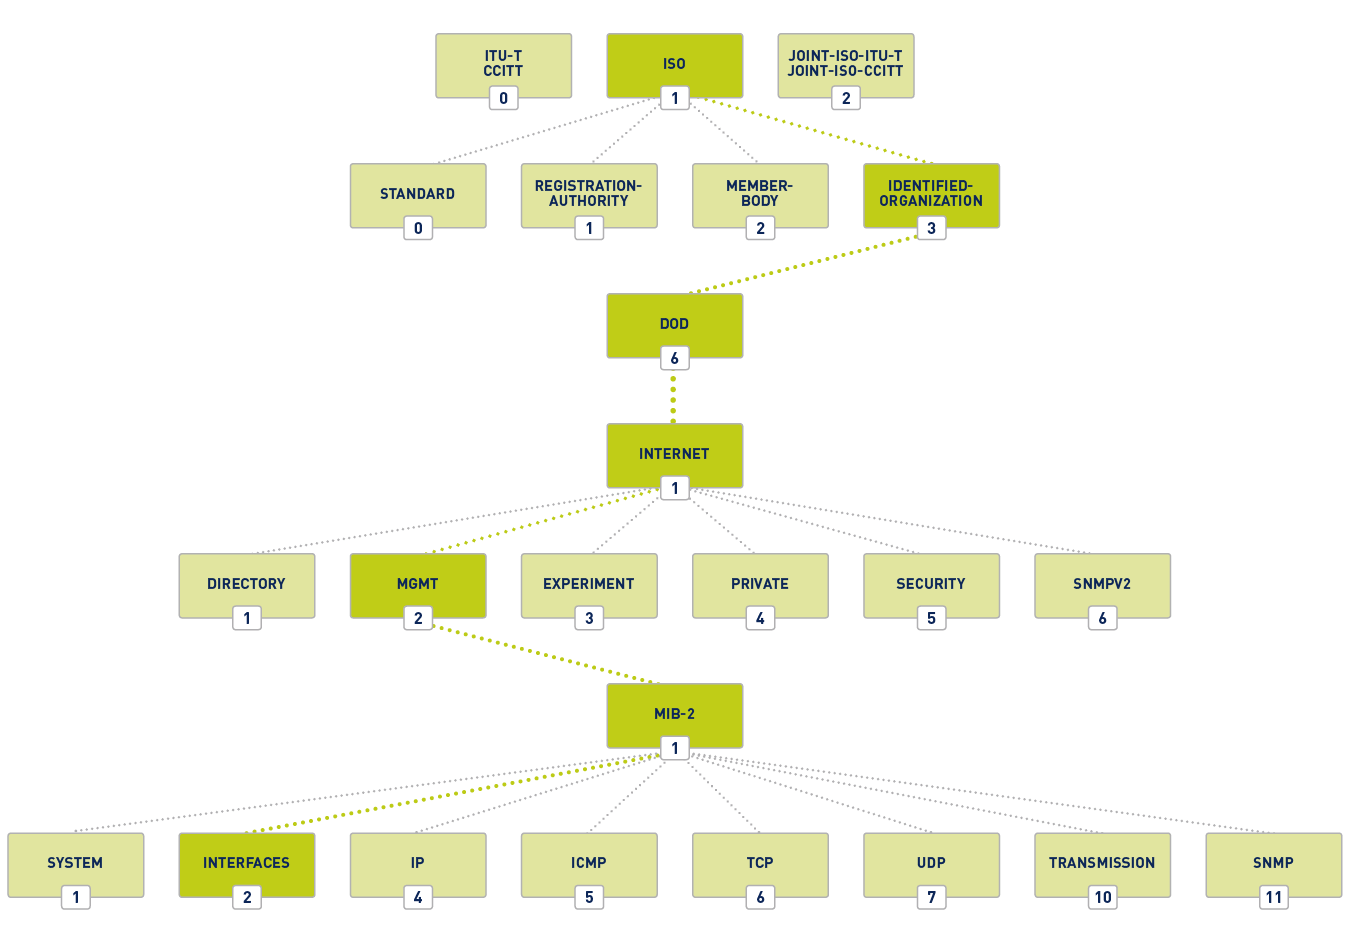
\includegraphics[ width=0.8\textwidth ]{pictures/OID-tree.png}
\end{figure}

\subsubsection{SNMPv2 configuration}

\begin{sexylisting}{SNMPv2 configuration}
snmp-server community batonaug ro SNMP_ACL

snmp-server enable traps
snmp-server host 192.168.1.3 version 2c batonaug

show snmp
\end{sexylisting}

The first command configures the community string, access level (read-only\code{ro},  read-write\code{rw}), and restrict SNMP access using ACL.The next two command enable traps and specify the recipient of the SNMP trap. By default, SNMP does not have any traps set. Without this command, SNMP managers must poll for all relevant information.

\subsection{SNMPv3 configuration}

SNMPv3 provides three security features: Message integrity and authentication, Encryption, Access control. The following commands show an example of basic SNMPv3 configuration:

\begin{sexylisting}{SNMPv3 configuration}
snmp-server view SNMP-RO iso included                                    
snmp-server group ADMIN v3 priv read SNMP-RO access PERMIT-ADMIN         
snmp-server user BOB ADMIN v3 auth sha cisco12345 priv aes 128 cisco54321
\end{sexylisting}

In the above example, the first command creates an SNMP view \code{SNMP-RO} and include the entire \code{iso} tree from the MIB. The next command creates an SNMP group \code{ADMIN}, the set to version 3 with authentication and encryption required. This command also gives read-only access to the view \code{SNMP-RO} to the group specified by the ACL called \code{PERMIT-ADMIN}. 

\section{NTP}

It is important to synchronize the time across all devices on the network because all aspects of managing, securing, troubleshooting, and planning networks require accurate time-stamping. Typically, the date and time settings on a router or switch can be set manually using \code{clock set} command, or by connecting NTP server via UDP port 123.\\

NTP networks use a hierarchical system of time sources. Each level in this hierarchical system is called a \textbf{stratum}. Smaller stratum numbers indicate that the server is closer to the authorized time source. Stratum 0 is the authoritative time sources (represented by the clock in the figure \ref{NTP}). Stratum 16, the lowest stratum level, indicates that a device is unsynchronized.\\

\begin{figure}[hbtp]
\caption{NTP Stratum levels}\label{NTP}
\centering
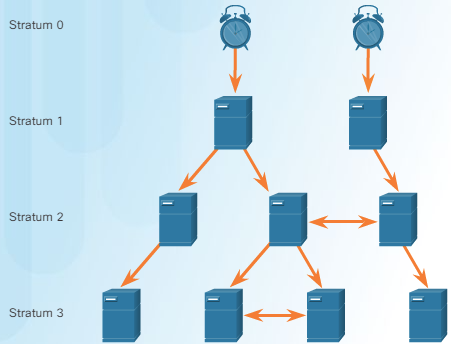
\includegraphics[ scale=0.7 ]{pictures/NTP.PNG}
\end{figure}

In the below configuration, the first command identifies NTP server.  The second command periodically updates the hardware clock with the time learned from NTP. The next commands configure NTP authentication on R1 using key 1 and password NTPpa55. To verify the system clock, use \code{show clock} command. To see if the device is synchronized with the NTP server, use \code{sh ip ntp ass} and \code{sh ntp status}.

\begin{sexylisting}{NTP authentication}
ntp server 192.168.1.5
ntp update-calendar

ntp authenticate
ntp trusted-key 1
ntp authentication-key 1 md5 NTPpa55

sh ntp status
sh ip ntp ass
sh clock
\end{sexylisting}

\section{Cisco AutoSecure}

AutoSecure makes recommendations for fixing security vulnerabilities and then modifies the security configuration of the router. It can lock down the functions of data and management plane. During AutoSecure setup, the following steps occur:

\begin{enumerate}
\item The AutoSecure command is entered
\item The wizard gathers info about the outside interfaces
\item Disable unnecessary services
\item Prompt for a security banner
\item Prompt for passwords and login features
\item Secure interface
\item Secure data plane
\end{enumerate}

Use the \code{auto secure} command to enable the Cisco AutoSecure feature setup. In interactive mode (default), the router prompts with options to enable and disable security features. On the other hand, the non-interactive mode (configured with the \code{auto secure no-interact} command) will automatically execute security features with default settings.

\section{Control plane security}

\subsection{Routing protocol authentication}

Routing Protocol Authentications mitigate against attacks like redirection of traffic to an insecure link, and redirection of traffic to discard it. OSPF supports routing protocol authentication using either MD5 or SHA.

\subsubsection{OSPF MD5 authentication}

\begin{sexylisting}{OSPF MD5 interface authentication}
interface s0/0/0
  ip ospf message-digest-key 1 md5 cisco12345
  ip ospf authentication message-digest
\end{sexylisting}

\begin{sexylisting}{OSPF MD5 area authentication}
router ospf 100
  area 50 authentication message-digest

interface s0/0/0
  ip ospf message-digest-key 1 md5 cisco12345
end
\end{sexylisting}

\note The interface setting overrides the global setting. OSPF adjacency is lost until MD5 authentication is matched between two routers.

\subsubsection{OSPF SHA authentication}

MD5 is now considered vulnerable to attacks. Therefore, the administrator should use SHA authentication. OSPF SHA authentication includes two major steps:

\begin{enumerate}
\item Specify an authentication key chain
\item Assign the authentication key to the desired interfaces 
\end{enumerate}

\begin{sexylisting}{OSPF SHA authentication}
key chain HUY
  key 1
  key-string cisco12345
  cryptographic-algorithm hmac-sha-256
  
interface s0/0/0
  ip ospf authentication key-chain HUY
\end{sexylisting}

\subsection{Control plane policing}

Routers must be able to distinguish between data plane, control plane, and management plane packets to treat each packet appropriately:

\begin{itemize}
\item \textbf{Data plane packets:} forward packets. Data plane are handled by CEF, which uses the control plane to pre-populate the FIB table. Subsequent packets that flow between same source and destination are forwarded by the data plane based on the information contained in the FIB.
\item \textbf{Control plane packets:} used for routing protocol (OSPF, EIGRP, BGP, etc.); sent to the router or network device
\item \textbf{Management plane packets:} used for management and reporting protocol (SSH, SNMP, NTP, etc.)
\end{itemize}